\chapter{Implementacija i korisničko sučelje}
		
		
		\section{Korištene tehnologije i alati}
					
					
			Članovi tima komunicirali su primarno putem aplikacije Whatsapp\footnote{https://www.whatsapp.com/}. WhatsApp je mobilna aplikacija za besplatnu razmjenu poruka, fotografija, videozapisa i drugih datoteka, te uspostavljanje glasovnih i videopoziva putem interneta. Komunikacija s asistenticom i demonstratorom ostvarena je aplikacijama Microsoft Teams\footnote{https://www.microsoft.com/en-us/microsoft-teams/group-chat-software} te Microsoft Outlook\footnote{https://www.microsoft.com/en-us/microsoft-365/outlook/}. Microsoft Teams je platforma za poslovnu komunikaciju, a Microsoft Outlook program za primanje i slanje elektroničke pošte. Oba proizvoda razvila je tvrtka Microsoft. Sastanci na daljinu također su održani putem aplikacije Microsoft Teams. Raspodjela zadataka i praćenje napretka ostvarena je pomoću Notiona\footnote{https://www.notion.so/}. Notion je aplikacija koja nudi organizacijske alate uključujući upravljanje zadacima, praćenje projekta, popise obaveza i označavanje.
			
			Dijagrami su izrađeni pomoću aplikacije Astah UML\footnote{https://astah.net/}, alata za UML modeliranje. Za izradu modela baze podataka korišten je alat ERDPlus\footnote{https://erdplus.com/}.
			
			Sustav korišten za upravljanje izvornim kodom je Git\footnote{https://git-scm.com/}, a udaljeni repozitorij projekta dostupan je na web platformi GitHub\footnote{https://github.com/}. GitHub služi za razvoj softvera i kontrolu verzija koja programerima omogućuje stvaranje, pohranu i upravljanje svojim kodom.
			
			Backend je pisan u programskom jeziku Java\footnote{https://www.java.com/}, pomoću radnog okvira Spring Boot\footnote{https://spring.io/}. Java je popularan objektno orijentiran programski jezik, a Spring Boot rješenje za stvaranje Spring aplikacija produkcijske razine s minimalnom količinom konfiguracije. Kao razvojno okruženje korišten je Intellij IDEA Ultimate\footnote{https://www.jetbrains.com/idea/download/}.
			
			Za razvoj frontenda korišteni su programski jezik JavaScript\footnote{https://www.javascript.com/} i biblioteka React\footnote{https://react.dev/}. Javascript je skriptni programski jezik koji se izvršava u web pregledniku na strani korisnika. React je njegova biblioteka otvorenog koda za izgradnju korisničkih sučelja temeljenih na komponentama. Razvojno okruženje je Visual Studio Code\footnote{https://code.visualstudio.com/}. 
			
			Lokalno pokrenuta web aplikacija koristi sustav za upravljanje bazama podataka H2\footnote{https://www.h2database.com/html/main.html}, dok aplikacija pogonjena pomoću platforme Render\footnote{https://render.com/} koristi sustav za upravljanje bazama PostgreSQL\footnote{https://www.postgresql.org/}. Razlika između H2 i PostgreSQL-a je u tome što H2 služi za testiranje i podaci se gube nakon gašenja sustava, a PostgreSQL trajno čuva podatke. 
			
			Za automatsko ispitivanje komponenti korišten je programski jezik Java i okvir JUnit 5\footnote{https://junit.org/junit5/}, a za automatsko ispitivanje sustava alat Selenium IDE\footnote{https://www.selenium.dev/selenium-ide/}. Selenium IDE omogućava snimanje, uređivanje i reproduciranje testova direktno u web pregledniku bez potrebe za pisanjem koda.
			
			Dokumentacija je pisana u programskom jeziku LaTeX\footnote{https://www.latex-project.org/}, u TeXstudiu\footnote{https://www.texstudio.org/}. TeXStudio je uređivač otvorenog koda namijenjen za LaTeX, programski jezik za pisanje strukturiranih tekstova i njihov automatski slog i prijelom u dokumente profesionalne kvalitete spremne za tisak.
						 
			
			\eject 
		
	
		\section{Ispitivanje programskog rješenja}
			
			\textbf{\textit{dio 2. revizije}}\\
			
			 \textit{U ovom poglavlju je potrebno opisati provedbu ispitivanja implementiranih funkcionalnosti na razini komponenti i na razini cijelog sustava s prikazom odabranih ispitnih slučajeva. Studenti trebaju ispitati temeljnu funkcionalnost i rubne uvjete.}
	
			
			\subsection{Ispitivanje komponenti}
			Programske komponente sastavljene su od nekoliko jedinica (najmanjih dijelova programa: razreda i pripadajućih metoda i atributa) s intenzivnom međusobnom interakcijom. Interakcija se ostvaruje putem proceduralnog sučelja gdje jedna komponenta enkapsulira skup funkcionalnosti koje mogu pozivati ostale komponente. Ispitivanje komponenti provedeno je  korištenjem Junit radnog okvira koji automatizira proces ispitivanja. Korištenjem dvije vrsta testova, normalnim načinom rada i unosom neispravnih i rubnih uvjeta, provjerava se očekivano ponašanje razreda i unaprijed definirani izlaz metode.
			
			Prilikom testiranja \texttt{UserService} metoda, korišteno je sučelje \texttt{UserRepository} uz klase \texttt{User} i \texttt{ProfileForm}. Najprije se testira funkcionalnost prijavljivanja u sustac. Prvi test provjerava uspješno prijavljivanje sa unaprijed zadanim korisničkim imenom. 
			
			
\begin{lstlisting}[xleftmargin=0em]
	@Test
	public void loginValidTest() {
		//Arrange
		newUser = new User();
		newUser.setUsername("Ivana");
		newUser.setEmail("ivana@gmail.com");
		newUser.setTypeOfUser("posjetitelj");
		newUser.setHomeAdress("adress");
		
		//Define mock behavior
		when(userRepository.findUserByUsername(
		newUser.getUsername())).thenReturn(newUser);
		
		//Actual test on service
		User savedUser = userService.login(newUser.getUsername());
		
		//Assertion
		assertNotNull(savedUser);
		assertEquals(newUser, savedUser);
	}
\end{lstlisting}			

			Drugi test provjerava prijavu u sustav sa neispravnim korisničkim imenom nakon što je zadano očekivano korisničko ime. 

\begin{lstlisting}[xleftmargin=0em]
	@Test
	public void loginInvalidTest() {
		//Arrange
		newUser = new User();
		newUser.setUsername("Ivana");
		
		//Define mock behavior
		lenient().when(userRepository.findUserByUsername(
		newUser.getUsername())).thenReturn(newUser);
		
		//Actual test on service
		User savedUser = userService.login("invalidUsername");
		
		//Assertion
		assertNull(savedUser);
		assertEquals(null,savedUser);
	}
	
\end{lstlisting}			
			
			
			Trećim testom provjeren je uspješan dohvat podataka o korisniku čiji su očekivani podatci unaprijed zadani. 
			
\begin{lstlisting}
	@Test
	public void retrieveUserDataTest() {
		// Arrange
		newUser = new User();
		newUser.setUsername("Ivana");
		newUser.setEmail("ivana@gmail.com");
		newUser.setTypeOfUser("posjetitelj");
		newUser.setHomeAdress("adress");
		
		// Define mock behavior
		when(userRepository.findUserByUsername(
		newUser.getUsername())).thenReturn(newUser);
		
		// Act
		profileForm = userService.data(newUser.getUsername());
		
		// Assert
		assertNotNull(profileForm);
		assertEquals(newUser.getUsername(), profileForm.getUsername());
		assertEquals("ivana@gmail.com", profileForm.getEmail());
		assertEquals("posjetitelj", profileForm.getTypeOfUser());
		assertEquals("adress", profileForm.getHomeAdress());
	}
\end{lstlisting}
			
			
			Provjerena je i promjena korisničkih podataka koja u sebi sadrži i provjeru prijave sa novim korisničkim podatcima.
			
\begin{lstlisting}
	@Test
	public void changeDataTest() {
		// Arrange
		Long userId = 1L;
		String newUsername = "newUsername";
		String newEmail = "newEmail@example.com";
		String newHomeAddress = "newAddress";
		
		User existingUser = new User();
		existingUser.setId(userId);
		existingUser.setUsername("oldUsername");
		existingUser.setEmail("oldEmail@example.com");
		existingUser.setHomeAdress("oldAddress");
		
		// Mock repository behavior
		when(userRepository.findUserById(userId)).thenReturn(existingUser);
		
		// Mock repository behavior for data update
		doAnswer(invocation -> {
			Long idArg = invocation.getArgument(0);
			String usernameArg = invocation.getArgument(1);
			String emailArg = invocation.getArgument(2);
			String homeAddressArg = invocation.getArgument(3);
			
			assertEquals(userId, idArg);
			assertEquals(newUsername, usernameArg);
			assertEquals(newEmail, emailArg);
			assertEquals(newHomeAddress, homeAddressArg);
			
			existingUser.setUsername(newUsername);
			existingUser.setEmail(newEmail);
			existingUser.setHomeAdress(newHomeAddress);
			
			return null;
		}).when(userRepository).updateUserById(anyLong(), anyString(), anyString(), anyString());
		
		
		// Act
		userService.changeData(userId, newUsername, newEmail, newHomeAddress);
		when(userRepository.findUserByUsername(
			existingUser.getUsername())).thenReturn(existingUser);
		User changedUser = userService.login(existingUser.getUsername());
		
		// Assert
		verify(userRepository, times(1)).updateUserById(userId, newUsername, newEmail, newHomeAddress);
		assertNotNull(changedUser);
	}
	
\end{lstlisting}

			Na kraju, provjereno je brisanje korisničkog profila uz pokušaj prijave sa obrisanim korisničkim podatcima.
			
\begin{lstlisting}
	@Test
	public void deleteMyProfileTest() {
		// Arrange
		Long userId = 1L;
		newUser = new User();
		newUser.setUsername("Ivana");
		newUser.setId(userId);
		
		// Mock repository behavior
		when(userRepository.findUserById(userId)).thenReturn(newUser);
		
		// Act
		userService.deleteMyProfile(userId);
		User deletedUser = userService.login(newUser.getUsername());
		
		// Assert
		verify(userRepository, times(1)).deleteUserById(userId);
		assertNull(deletedUser);
		assertEquals(null, deletedUser);
		
	}
\end{lstlisting}

			Na slici \ref{komp} prikazan je rezultat izvođenja navedenih testova. 
			
			\begin{figure}[H]
				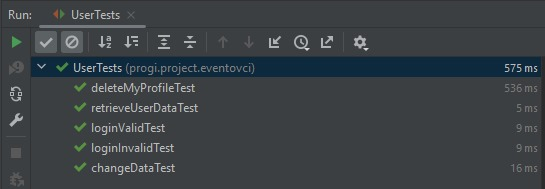
\includegraphics[width=\textwidth]{slike/ispitivanje_komponenti.jpeg} 
				\centering
				\vspace{-0.2cm}
				\caption{Svi su testovi ispravno izvedeni}
				\label{komp}
			\end{figure}
			
			
			
			\subsection{Ispitivanje sustava}
			
			 Ispitivanje cijelog sustava napravljeno je pomoću Selenium WebDrivera unutar Junit testova. U svakom od testova unaprijed definiramo postavke drivera uz zadavanje URL-a aplikacije. Driver zatim sam pronalazi unaprijed zadane elemente, a putem testa prosljeđuju mu se podatci. Najprije je testirano ispravno prijavljivanje u sustav unaprijed registriranog korisnika. Budući da su podatci ispravni, aplikacija preusmjerava korisnika na početnu stranicu.
			 
\begin{lstlisting}
	@Test
	public void loginValidTest() throws InterruptedException {
		
		driver.get("https://eventovci.onrender.com/login");
		
		WebElement element = driver.findElement(By.id("nameField"));
		element.sendKeys("registeredUserr");
		element = driver.findElement(By.id("sifrafild"));
		element.sendKeys("password");
		
		driver.findElement(By.cssSelector("button[type='submit']")).click();
		Thread.sleep(5000);
		
		String url = driver.getCurrentUrl();
		driver.quit();
		Assertions.assertEquals("https://eventovci.onrender.com/home", url);
	}
	
\end{lstlisting}

			Drugi test provjerava neispravnu prijavu (pogrešna lozinka) zbog čega driver na kraju testa ostaje na stranici za prijavu.
			
\begin{lstlisting}
	@Test
	public void loginInvalidTest() throws InterruptedException {
		
		driver.get("https://eventovci.onrender.com/login");
		
		WebElement element = driver.findElement(By.id("nameField"));
		element.sendKeys("registeredUserr");
		element = driver.findElement(By.id("sifrafild"));
		element.sendKeys("wrongPassword");
		
		driver.findElement(By.cssSelector("button[type='submit']")).click();
		Thread.sleep(5000);
		
		String url = driver.getCurrentUrl();
		driver.quit();
		Assertions.assertEquals("https://eventovci.onrender.com/login", url);
	}
\end{lstlisting}

			Trećim testom provjereno je uspješno registriranje korisnika kao posjetitelja. Nakon registracije, korisnika se preusmjerava na početnu stranicu.
			
\begin{lstlisting}
	@Test
	public void registerValidTest() throws InterruptedException {
		
		driver.get("https://eventovci.onrender.com/login");
		
		driver.findElement(By.cssSelector("button")).click();
		Thread.sleep(5000);
		
		WebElement element = driver.findElement(By.id("nameField"));
		element.sendKeys("NewUserRegisterrr");
		element = driver.findElement(By.id("sifrafild"));
		element.sendKeys("password");
		element = driver.findElement(By.id("email-field"));
		element.sendKeys("NewUserRegisterrr@gmail.com");
		
		driver.findElement(By.cssSelector("button[type='submit']")).click();
		Thread.sleep(5000);
		
		String url = driver.getCurrentUrl();
		driver.quit();
		Assertions.assertEquals("https://eventovci.onrender.com/home", url);
	}
\end{lstlisting}

			Ukoliko korisnik ne unese pravilno podatke za registraciju, ostat će na stranici za prijavu uz ispis greške koju treba popraviti (korisničko ime već postoji, e-mail nije u pravilnom formatu...) što se ispituje četvrtim testom.
			
\begin{lstlisting}
	@Test
	public void registerInvalidTest() throws InterruptedException {
		
		driver.get("https://eventovci.onrender.com/login");
		
		driver.findElement(By.cssSelector("button")).click();
		Thread.sleep(5000);
		
		WebElement element = driver.findElement(By.id("nameField"));
		element.sendKeys("registerNewUserr");
		element = driver.findElement(By.id("sifrafild"));
		element.sendKeys("password");
		element = driver.findElement(By.id("email-field"));
		element.sendKeys("registerNewUser-wrongMail");
		
		driver.findElement(By.cssSelector("button[type='submit']")).click();
		Thread.sleep(5000);
		
		String url = driver.getCurrentUrl();
		driver.quit();
		Assertions.assertEquals("https://eventovci.onrender.com/login", url);
	}
\end{lstlisting}

			Posljednji test sustava provjerava dodavanje novog događanja. Nakon što se unaprijed registriran korisnik prijavi sa svojim podatcima, pokušat će dodati novi događaj uz izostanak postavljanja cijene. Dodavanje se neće uspješno provesti te korisnik ostaje na stranici za dodavanje događaja uz ispis odgovarajuće poruke. 
			
\begin{lstlisting}
	@Test
	public void addNewEventInvalid() throws InterruptedException {
		
		driver.get("https://eventovci.onrender.com/login");
		WebElement element = driver.findElement(By.id("nameField"));
		element.sendKeys("eventCoordinator");
		element = driver.findElement(By.id("sifrafild"));
		element.sendKeys("password");
		
		driver.findElement(By.cssSelector("button[type='submit']")).click();
		Thread.sleep(5000);
		
		driver.findElement(By.cssSelector("div.category img[alt='img for MOJ RACUN']")).click();
		
		String url = driver.getCurrentUrl();
		Assertions.assertEquals("https://eventovci.onrender.com/my-account", url);
		
		driver.findElement(By.xpath("//button[text()='Dodaj dogadanje']")).click();
		
		url = driver.getCurrentUrl();
		Assertions.assertEquals("https://eventovci.onrender.com/add-event", url);
		
		driver.findElement(By.id("nameField")).sendKeys("Event Name");
		driver.findElement(By.id("typeField")).sendKeys("Koncert");
		driver.findElement(By.id("locationField")).sendKeys("Centar");
		driver.findElement(By.id("timeField")).sendKeys("2024-01-15T12:00");
		driver.findElement(By.id("durationField")).sendKeys("02:00");
		//driver.findElement(By.id("priceField")).sendKeys("0");
		driver.findElement(By.xpath("//textarea")).sendKeys("Event Description");
				
		driver.findElement(By.cssSelector("button.dodaj-dogadjanje")).click();
		Thread.sleep(5000);
		
		url = driver.getCurrentUrl();
		driver.quit();
		Assertions.assertEquals("https://eventovci.onrender.com/add-event", url);
	}
\end{lstlisting}

			Na slici \ref{sust} prikazan je rezultat izvođenja navedenih testova.

			\begin{figure}[H]
				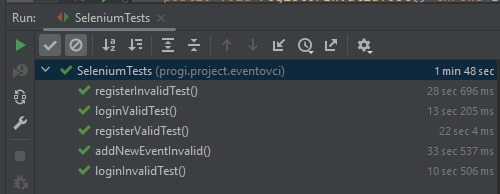
\includegraphics[width=\textwidth]{slike/ispitivanje_sustava.jpeg} 
				\centering
				\vspace{-0.2cm}
				\caption{Dijagram razmještaja}
				\label{sust}
			\end{figure}
			
			
			\eject 
		
		
		\section{Dijagram razmještaja}
		
			Na slici \ref{depd} prikazan je specifikacijski dijagram razmještaja. Funkcioniranje sustava temelji se na arhitekturi poznatoj kao "klijent-poslužitelj". Korisnici (posjetitelji, organizatori, administrator) pristupaju web aplikaciji korištenjem web preglednika na svom računalu. Web poslužitelj i poslužitelj baze podataka nalaze se na poslužiteljskom računalu. Web aplikacija odgovorna je i za uspostavu veze i komunikaciju s bazom podataka. Interakcija između računala korisnika i poslužitelja ostvaruje se putem HTTP veze.
			
			
			\begin{figure}[H]
				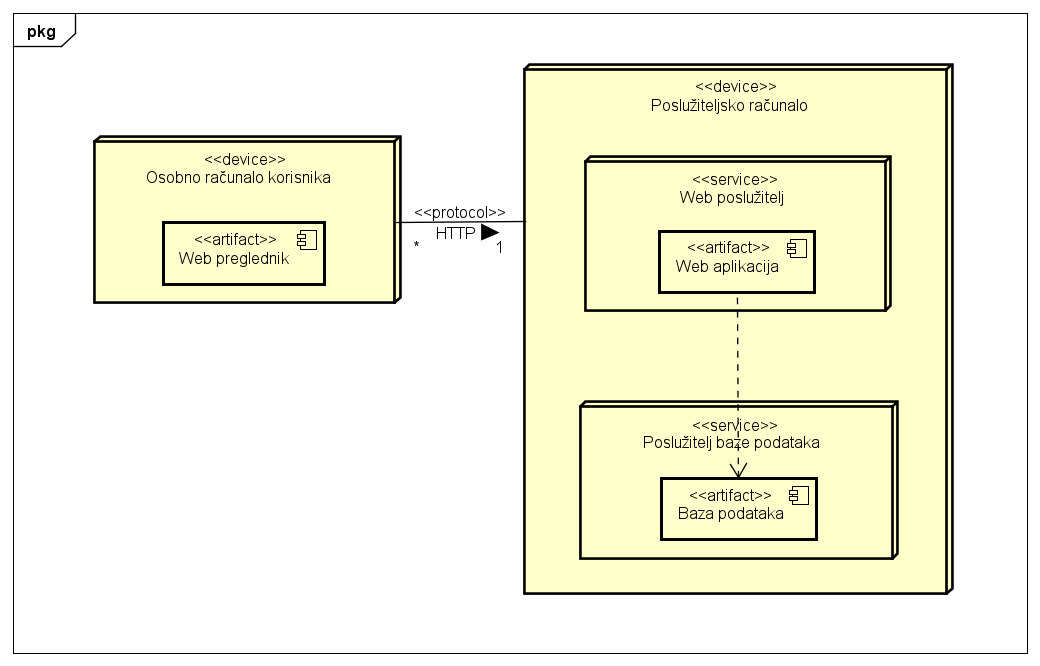
\includegraphics[width=\textwidth]{dijagrami/depd.png} 
				\centering
				\vspace{-0.2cm}
				\caption{Dijagram razmještaja}
				\label{depd}
			\end{figure}
			
			
			\eject 
		
		\section{Upute za puštanje u pogon}
		
			
			\textit{Za deploy aplikacije korištena je platforma Render. Putem njega omogućeno je da aplikacija bude javno dostupna. Pri implementaciji web usluge na render najprije je s njime potrebno povezati svoj GitHub repozitorij, pripremiti projekt za deploy te kreirati potrebne dijelove na Render-u.}
			
			\subsection{Priprema projekta za deploy}
			\textit{Priprema projekta za deploy na Render uključuje pripremu backenda i pripremu frontenda. Za pripremu backenda potrebno je dodati varijable okruženja, dodati DockerFile te postaviti /api kao prefiks svim zahtjevima na backend, dok je za pripremu frontenda potrebno dodati dependencye u package.json, dodati /src/setupProxy.js koji služi kao proxy server za lokalni development te dodati app.js u kojem se nalazi express server za posluživanje frontenda. Zatim je potrebno u Rander kontolnoj ploči kreirati bazu podataka, backend i fronted.}
			
			\subsection{Kreiranje potrebnih dijelova na Render-u}
			\textit{Prvo kreiramo bazu podataka tako što odaberemo opciju Novo -> PostgreSQL u Renderovoj kontrolnoj ploči. Postavimo ime baze i korisničko ime te kliknemo Stvori Bazu podataka. Zatim kreiramo backend tako što odaberemo Novo -> Web Service. Ukoliko nismo povezali račun sada moramo kako bi mogli odabrati projekt kojeg želimo deployati. Nakon toga sve što je potrebno je postaviti ime za servis koje postaje dio web adrese, postavitit korijennski direktorij, dodati potrebne varijable okruženja (tj. kopirati njihove vrijednosti iz postavki baze podataka na Renderu), za environment odabrati Docker te postaviti putanju za Dockerfile. Tada odaberemo stvoriti Web uslugu. Posljednji korak je kreiranje frontenda pomoću odabira Novo -> Web Service. Zatim se odabire projekt, ime za servis, postavi korijenski direktorij, za environment odabire Node te za region Frankfurt, postavljamo komande upravljanja i dodamo potrebne varijable okruženja. Tada odaberemo stvoriti Web Service.
			
			
			\eject 